
\section{Word Embedding Experiments}
\label{sec:experiments}

Using the parameter selections outlined in Section \ref{sec:training}, we perform a partial parameter sweep over the various preprocessing techniques, normalization options, and word2vec parameterizations to determine the optimal word embedding methods. The text corpus for training the embeddings is an Arabic Wikipedia dump from \url{https://dumps.wikimedia.org/arwiki/20150901/} \cite{wiki:xxx}, cleaned by dropping Wikipedia markup, punctuation, and non-Arabic characters. All preprocessing options are precomputed first, generating multiple versions of the Arabic Wikipedia corpus. Then word vectors are trained for each parameterization. The vectors are then ran through the evaluation tasks, recording performance statistics.

\subsection{Word Similarity 353}

The results for English vectors on the semantic similarity tasks are shown in Table \ref{table:englishtask} for comparison. There are two models shown, each evaluated on the WS353 English word similarity task. The first is an English model trained under the default Word2Vec parameterization (skipgram, window of 7, 100 dimensions) on the same number of words as our Arabic models. The second is the publically available pre-trained vectors trained on a 100 billion word Google News Corpus \cite{mikolovdist:2013}. The metric that we choose to base our evaluate on is the Spearman correlation between the model similarity estimates the evaluation task similarity values. \textcolor{red}{We also provide the mean squared error as the mean squared difference between the model estimate and the evaluation task value. The default vectors exhibit an impressive .268 MSE, and} both models show a high correlation with the evaluation task scores. The Google News vectors display an impressive $.6978$ Spearman correlation score to the task, providing a high score to aim for. We consider the $0.5457$ correlation score of the default English task to be the baseline for our Arabic word embeddings.

\begin{table}
\begin{tabular}{l|l|l}
\bfseries Method &\bfseries Similarity Correlation & \bfseries Analogy Accuracy
\csvreader[head to column names]{results_spearman/en_prepared_hybrid.csv}{}
{\\\hline\csvcoli&\Spearman&\Scores}
\end{tabular}
\caption{English Baseline Results}
\label{table:englishtask}
\end{table}

Table \ref{table:ws353task} shows the results of the models with the 10 highest correlation scores on the Word Similarity 353 task \cite{finkelstein:2001,hassan:2009}. \textcolor{red}{Do these tables add?} Standing out is the lack of any preprocessing method but tokenization in this list. Additionally, these best performing models were primarily trained using a window of 4 words. Figure \ref{fig:spearplotws353} shows box plots over all results grouped by the two most significant preprocessing measures, Window size and Preprocessing method. These results show that tokenization is the only method not only as good as teh English baseline, but able to perform better. This improvement can be considered even more significant due to the translation of the task, but it is difficult to quantify this effect. Interestingly, the unprocessed Arabic scores higher than lemmatization on this task. textcolor{red}{Interpret.} The window size is very interesting, as this parameter is highly dependent on the grammar of the training language. A sentence structure that uses complex words more often has related words nearer to each other than English does, so Arabic word embeddings may benefit from having a smaller window to not look beyond the relevant information.

\begin{table}
\begin{tabular}{l|l|l|l|l}
\bfseries Rank & \bfseries Preprocessing & \bfseries Window & \bfseries Size & \bfseries Correlation
\csvreader[column count=15,head to column names]{results_spearman/ar_similiarity_task_results_ws353_prepared.csv}{}
{\\\hline\rank&\preprocessing&\wind&\size&\Spearman}
\end{tabular}
\caption{Top Results on Word Similarity 353}
\label{table:ws353task}
\end{table}

\begin{figure}
  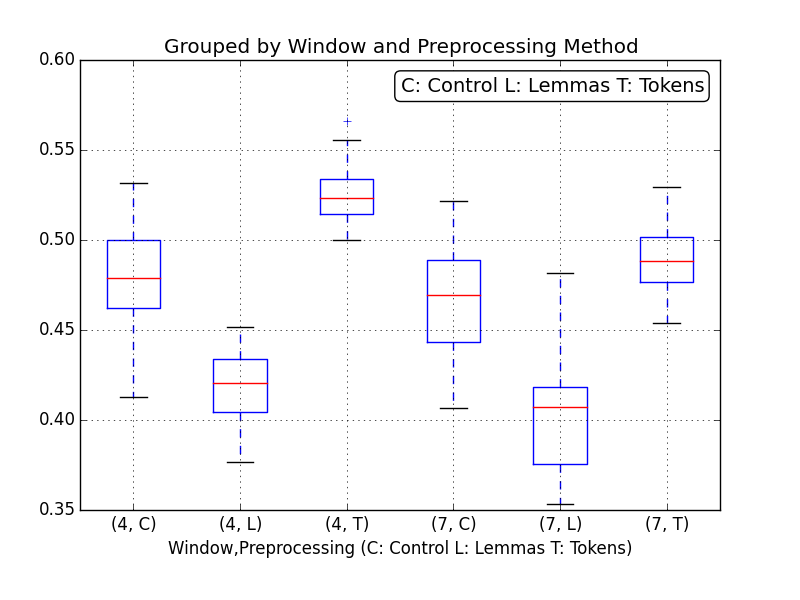
\includegraphics[width=\linewidth]{results_spearman/ar_similiarity_task_results_ws353_spearplot.png}
  \caption{WS353 Results}
  \label{fig:spearplotws353}
\end{figure}

\subsection{Our Similarity Task}

Table \ref{table:ourtask} shows the results of the models with the 10 highest correlation scores on the task we developed \textcolor{red}{Pick one of the three model options. The subset with 4 votes has the highest correlation but only ~250 word pairs.} The results on our data support our findings that the smaller window size does indeed have a strong positive impact on the quality of the word embeddings. \textcolor{red}{We suspect that the high performance of the control group without preprocessing is due to the evaluation task being developed from the same corpus as the vector training data. Interpret, verify?}

% Embedding File,MSE,Accuracy,Hit_Percent,Correlation,Correlation Sig,Spearman,Spearman Sig,wind,size,mod,dig,tash,preprocessing
% 1              2    3        4            5          6           7    8        9           10   11   12  13  14   15

\begin{table}
\begin{tabular}{l|l|l|l|l}
\bfseries Rank & \bfseries Preprocessing & \bfseries Window & \bfseries Size & \bfseries Correlation
\csvreader[head to column names]{results_spearman/ar_similiarity_task_results_prepared.csv}{}
{\\\hline\rank&\preprocessing&\wind&\size&\Spearman}
\end{tabular}
\caption{Top Results on our whole Task}
\label{table:ourtask}
\end{table}

\begin{table}
\begin{tabular}{l|l|l|l|l}
\bfseries Rank & \bfseries Preprocessing & \bfseries Window & \bfseries Size & \bfseries Correlation
\csvreader[head to column names]{results_spearman/ar_similiarity_task_multi_results_prepared.csv}{}
{\\\hline\rank&\preprocessing&\wind&\size&\Spearman}
\end{tabular}
\caption{Top Results on our Task-2+ Votes}
\label{table:ourtaskmulti}
\end{table}

\begin{table}
\begin{tabular}{l|l|l|l|l}
\bfseries Rank & \bfseries Preprocessing & \bfseries Window & \bfseries Size & \bfseries Correlation
\csvreader[head to column names]{results_spearman/ar_similiarity_task_4_votes_results_prepared.csv}{}
{\\\hline\rank&\preprocessing&\wind&\size&\Spearman}
\end{tabular}
\caption{Top Results on our Task-4 Votes}
\label{table:ourtask4}
\end{table}

\begin{figure}
  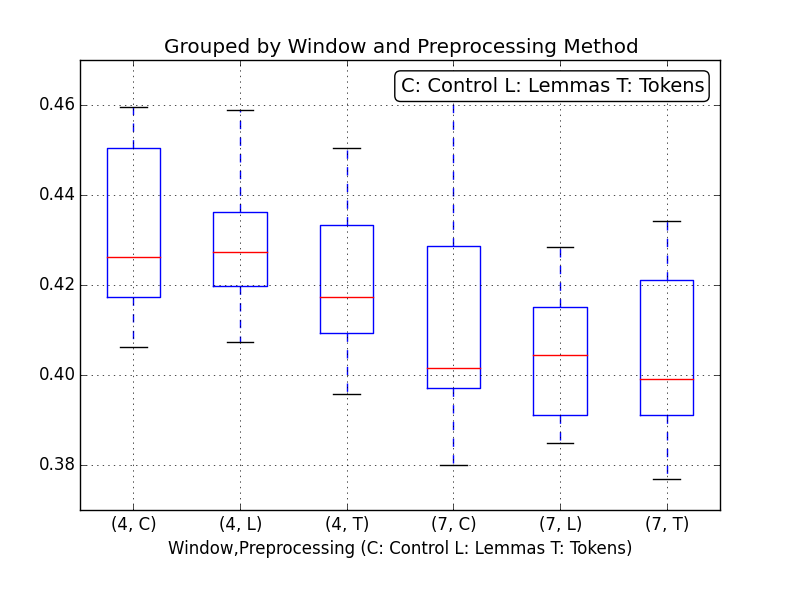
\includegraphics[width=\linewidth]{results_spearman/ar_similiarity_task_results_spearplot.png}
  \caption{Our Whole Task Results}
  \label{fig:spearplot1}
\end{figure}

\begin{figure}
  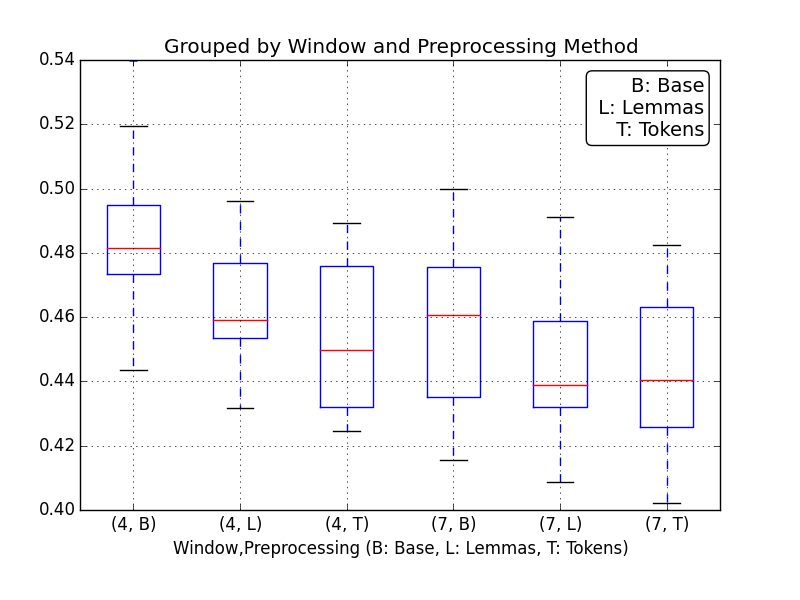
\includegraphics[width=\linewidth]{results_spearman/ar_similiarity_task_multi_results_spearplot.png}
  \caption{Our Task 2+ Votes Results}
  \label{fig:spearplot2}
\end{figure}

\begin{figure}
  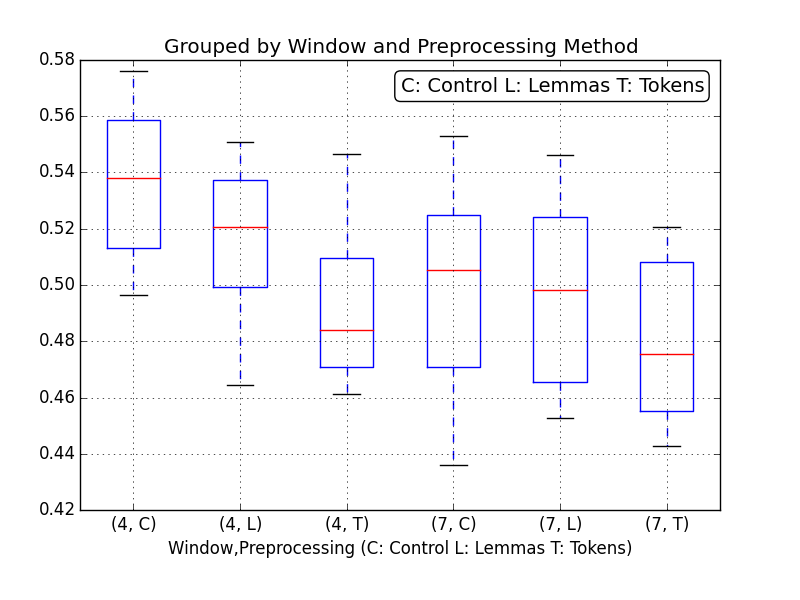
\includegraphics[width=\linewidth]{results_spearman/ar_similiarity_task_4_votes_results_spearplot.png}
  \caption{Our Task 4 Votes Results}
  \label{fig:spearplot4}
\end{figure}

% full/4: tau: 0.334649122807, p_value: 1.36433095045e-06
% multi/full: tau: 0.481578947368, p_value: 3.63086505503e-12
% multi/4: tau: 0.572368421053, p_value: 1.44144439867e-16

We have shown that preprocessing and training decisions can substantially change the performance of Arabic word embeddings on similarity tasks. Some methods were even able to surpass the English baseline. While the best performing models were still significantly below the scores of the English embeddings trained on the Google News corpus, this is to be expected considering the strong correlation between the quantity of training data and the quality of the word embeddings. Our training set has approximately 5 million Arabic words while the Google News set has about 100 billion words \cite{mikolovdist:2013}.

\subsection{Analogy Task}

Table \ref{table:englishanalogy} shows the baseline results of the English embeddings on the Analogy task. These results demonstrate the extreme difference in quality between vectors trained on 5 million words and 100 billion words. The lower accuracy of the 5 million word model at $0.04522$, or 4.522 percent correct of the $19544$ analogies, will be used as a comparitive baseline for this task.


\begin{table}
\begin{tabular}{l|l}
\bfseries Model & \bfseries Accuracy
\csvreader[head to column names]{results_analogy/en_prepared.csv}{}
{\\\hline\csvcoli&\csvcoliii}
\end{tabular}
\caption{English Analogy Results}
\label{table:englishanalogy}
\end{table}

% Embedding File,Hit_Percent,Scores,wind,size,mod,dig,tash,preprocessing
% 1               2           3      4   5      6 7    8   9

Table \ref{table:aranalogy} shows the top 10 analogy task results from the Arabic models. Here it seems models preprocessed to lemmas and trained to 200 dimensions seem to dominate. We also see less difference between models with different window sizes. Figure \ref{fig:aranalogy} confirms these trends with boxplots with groups by significant factors. This plot illustrates the dramatic improvements that are obtained with proper preprocessing and parameterization for the task. The lemmatized 200 dimensional models consistently outperformed all other models, including the baseline English model. In the best case, one ideally parameterized model is nearly 50\% better than the English baseline. Of lesser note, the tokenization method also delivers significantly higher accuracies than the models that received no preprocessing on the Arabic. These results demonstrate that preprocessing and training decisions can greatly improve the performance of Arabic word embeddings on analogy solving tasks, improving scores from as low as half of the English baseline to as high as 150\% of the baseline.

\begin{table}
\begin{tabular}{l|l|l|l|l}
\bfseries Rank & \bfseries Preprocessing & \bfseries Window & \bfseries Size & \bfseries Accuracy
\csvreader[head to column names]{results_analogy/ar_analogy_results_fixed_prepared.csv}{}
{\\\hline\rank&\csvcolix&\csvcoliv&\csvcolx&\csvcoliii}
\end{tabular}
\caption{Top Results on Arabic Analogy Task}
\label{table:aranalogy}
\end{table}

\begin{figure}
  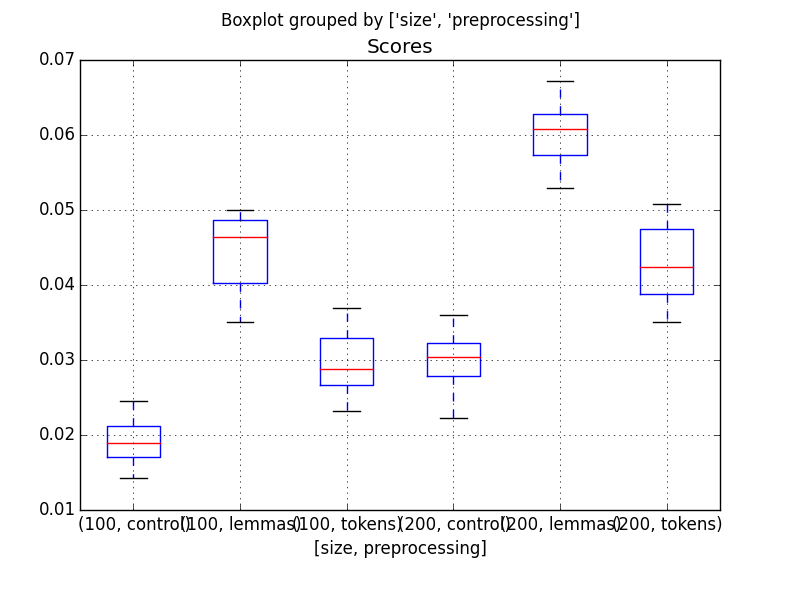
\includegraphics[width=\linewidth]{results_analogy/ar_analogy_results_fixed_plot.png}
  \caption{Arabic Analogy Task Results}
  \label{fig:aranalogy}
\end{figure}















